%
% Categorifying the zx-calculus
% SMCC Structure
% arXiv v2
%

\documentclass[./1--Catfying_zxCalc--Master.tex]{subfiles} % ./mainfilename.tex
%\input{Catfying_zxCalc--Preamble.tex}

%%%%%%%%%%%%%%%%%%%%
%%%%%%%%%%%%%%%%%%%%
%
% BEGIN DOCUMENT
\begin{document}
%
%%%%%%%%%%%%%%%%%%%%
%%%%%%%%%%%%%%%%%%%%

%%%%%%%%%%%%%%%%%%%%
\section{A symmetric monoidal bicategory of spans of cospans}
\label{sec:SMCC Bicat SpCsp}
%%%%%%%%%%%%%%%%%%%%

In this section, 
we prove Theorem 
	\ref{thm:SpCspC is SMCC bicategory}. 
Let $\cat{C} = (\cat{C}_0, \otimes, I)$ be 
a finitely complete and cocomplete 
(braided, symmetric) monoidal category 
such that $\otimes$ preserves colimits. 
The category $\cat{Graph}$ together
with its coproduct is one example.
The proof consists of two parts: 
that $\spcsp{C}$ is a (braided, symmetric) 
monoidal bicategory and 
that it is compact closed.

We first show $\spcsp{C}$ 
is a (braided, symmetric) 
monoidal bicategory 
with a result from Shulman. 

\begin{thm}{\cite[Theorem 5.1]{Shulman_ConstructSMBicats}}
	\label{thm:DoubleGivesBi}
	Let $\dblcat{D}$ be an 
	isofibrant (braided, symmetric) 
	monoidal double category. 
	There is a (braided, symmetric) 
	monoidal bicategory $\cat{D}$ 
	whose objects are those of $\dblcat{D}$ 
	and whose hom-categories $\cat{D}(x,y)$ 
	have as 
	objects the horizontal arrows 
	in $\dblcat{D}$ of type $x \to y$ 
	and as morphisms the 
	2-cells in $\dblcat{D}$ of type
	\[
	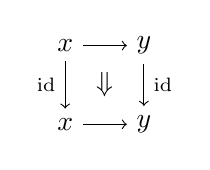
\begin{tikzpicture}
		\node (1) at (0,1) {$x$};
		\node (2) at (1,1) {$y$};
		\node (3) at (1,0) {$y$};
		\node (4) at (0,0) {$x$};
		\node at (0.5,0.5) {$\Downarrow$};
		\draw [->] (1) to (2);
		\draw [->] (1) to node[left] {\scriptsize id} (4);
		\draw [->] (2) to node[right] {\scriptsize id} (3);
		\draw [->] (4) to (3);
	\end{tikzpicture}
	\]
\end{thm}

The same paper 
	\cite{Shulman_ConstructSMBicats} 
also contains the definitions used in this section.  
To use this theorem, we begin construction 
on a double category $\dblspcsp{C}$. 
This requires \emph{cubical spans of cospans}, 
which are commuting diagrams of shape 
\[
\begin{tikzpicture}
	\node (A) at (0,2) {$\bullet$};
	\node (A') at (0,1) {$\bullet$};
	\node (A'') at (0,0) {$\bullet$};
	\node (B) at (1,2) {$\bullet$};
	\node (B') at (1,1) {$\bullet$};
	\node (B'') at (1,0) {$\bullet$};
	\node (C) at (2,2) {$\bullet$};
	\node (C') at (2,1) {$\bullet$};
	\node (C'') at (2,0) {$\bullet$};
	%
	\path[->,font=\scriptsize,>=angle 90]
	% horizontal arrows
	(A) edge node{} (B)
	(A') edge node{} (B')
	(A'') edge node{} (B'')
	(C) edge node{} (B)
	(C') edge node{} (B')
	(C'') edge node{} (B'')
	% vertical arrows
	(A') edge node{} (A)
	(A') edge node{} (A'')
	(B') edge node{} (B)
	(B') edge node{} (B'')
	(C') edge node{} (C)
	(C') edge node{} (C'');
\end{tikzpicture}
\]
We get an equivalence relation on these 
by relating cubical spans of cospans 
that share the same outside square.
The induced classes are called
\emph{parallel classes}.

% DOUBLE CATEGORIES
\begin{lem}
	\label{lem:SpanCospanDoubleCat}
	There is a double category $\dblspcsp{C}$ 
	whose objects are the $\cat{C}$-objects, 
	vertical morphisms are given by 
	isomorphism classes of spans in $\cat{C}$ with invertible legs, 
	horizontal morphisms are given by cospans in $\cat{C}$, 
	and 2-morphisms are parallel classes of 
	cubical spans of cospans in $\cat{C}$. 
\end{lem}

\begin{proof}
	Define the object category 
	$\widetilde{\dblcat{C}}_0$ 
	to have as objects 
	the $\cat{C}$-objects and 
	as morphisms the isomorphism classes of 
	spans in $\cat{C}$ with invertible legs. 
	Define the arrow category 
	$\widetilde{\dblcat{C}}_1$ 
	to have as objects the 
	cospans in $\cat{C}$ and 
	as morphisms the 
	parallel classes of 
	cubical spans of cospans 
	in $\cat{C}$.  
	
	The structure functor 
		$U \from \widetilde{\dblcat{C}}_0 \to \widetilde{\dblcat{C}}_1$ 
	acts on objects by 
	mapping $x$ to the identity cospan on $x$ 
	and on morphisms by 
	mapping $x \gets y \to z$, whose legs are isomorphisms, 
	to 
	\[
	\begin{tikzpicture}
	\node (A) at (0,2) {$x$};
	\node (A') at (0,1) {$x$};
	\node (A'') at (0,0) {$x$};
	\node (B) at (1,2) {$y$};
	\node (B') at (1,1) {$y$};
	\node (B'') at (1,0) {$y$};
	\node (C) at (2,2) {$z$};
	\node (C') at (2,1) {$z$};
	\node (C'') at (2,0) {$z$};
	%
	\path[->,font=\scriptsize,>=angle 90]
	% horizontal arrows
	(A) edge node{} (B)
	(A') edge node{} (B')
	(A'') edge node{} (B'')
	(C) edge node{} (B)
	(C') edge node{} (B')
	(C'') edge node{} (B'')
	% vertical arrows
	(A') edge node{} (A)
	(A') edge node{} (A'')
	(B') edge node{} (B)
	(B') edge node{} (B'')
	(C') edge node{} (C)
	(C') edge node{} (C'');
	\end{tikzpicture}
	\]
	The source functor 
		$S \from \widetilde{\dblcat{C}}_1 \to \widetilde{\dblcat{C}}_0$ 
	acts on objects by sending 
	$x \to y \gets z$ to $x$ and 
	on morphisms by sending 
	a cubical span of cospans to the span 
	occupying the left vertical side.  
	The target functor $T$ is defined similarly.  
	
	The horizontal composition functor 
		$\odot \from 
			\widetilde{\dblcat{C}}_1 \times_{\widetilde{\dblcat{C}}_0} \widetilde{\dblcat{C}}_1 \to \widetilde{\dblcat{C}}_1$ 
	acts on objects by 
	composing cospans with pushouts 
	in the usual way.  
	It acts on morphisms by 
	\[
	\raisebox{-0.5\height}{
		\begin{tikzpicture}
		\node (A) at (0,2) {$a$};
		\node (A') at (0,1) {$a'$};
		\node (A'') at (0,0) {$a''$};
		\node (B) at (1,2) {$b$};
		\node (B') at (1,1) {$b'$};
		\node (B'') at (1,0) {$b''$};
		\node (C) at (2,2) {$c$};
		\node (C') at (2,1) {$c'$};
		\node (C'') at (2,0) {$c''$};
		\node (D) at (3,2) {$d$};
		\node (D') at (3,1) {$d'$};
		\node (D'') at (3,0) {$d''$};
		\node (E) at (4,2) {$e$};
		\node (E') at (4,1) {$e'$};
		\node (E'') at (4,0) {$e''$};
		%
		\path[->,font=\scriptsize,>=angle 90]
		% horizontal arrows
		(A) edge node[above]{} (B)
		(A') edge node[above]{} (B')
		(A'') edge node[above]{} (B'')
		(C) edge node[above]{} (B)
		(C') edge node[above]{} (B')
		(C'') edge node[above]{} (B'')
		(C) edge node[above]{} (D)
		(C') edge node[above]{} (D')
		(C'') edge node[above]{} (D'')
		(E) edge node[above]{} (D)
		(E') edge node[above]{} (D')
		(E'') edge node[above]{} (D'')
		% vertical arrows
		(A') edge node[left]{} (A)
		(A') edge node[left]{} (A'')
		(B') edge node[left]{} (B)
		(B') edge node[left]{} (B'')
		(C') edge node[left]{} (C)
		(C') edge node[left]{} (C'')	
		(D') edge node[left]{} (D)
		(D') edge node[left]{} (D'')
		(E') edge node[left]{} (E)
		(E') edge node[left]{} (E'');
		\end{tikzpicture}
	}
	\quad
	\xmapsto[]{\odot}
	\quad
	\raisebox{-0.5\height}{
		\begin{tikzpicture}
		\node (A) at (0,2) {$a$};
		\node (A') at (0,1) {$a'$};
		\node (A'') at (0,0) {$a''$};
		\node (B) at (1.5,2) {$b+_{c}d$};
		\node (B') at (1.5,1) {$b'+_{c'}d'$};
		\node (B'') at (1.5,0) {$b''+_{c''}d''$};
		\node (C) at (3,2) {$e$};
		\node (C') at (3,1) {$e'$};
		\node (C'') at (3,0) {$e''$};
		%
		\path[->,font=\scriptsize,>=angle 90]
		% horizontal arrows
		(A) edge node[above]{} (B)
		(A') edge node[above]{} (B')
		(A'') edge node[above]{} (B'')
		(C) edge node[above]{} (B)
		(C') edge node[above]{} (B')
		(C'') edge node[above]{} (B'')
		% vertical arrows
		(A') edge node[left]{} (A)
		(A') edge node[left]{} (A'')
		(B') edge node[left]{} (B)
		(B') edge node[left]{} (B'')
		(C') edge node[left]{} (C)
		(C') edge node[left]{} (C'');	
		\end{tikzpicture}
	}
	\]
	This respects identities and 
	we separate the proof that 
	$\odot$ respects composition 
	into the next lemma.  
	It is straightforward to check 
	that the required equations are satisfied.  
	The associators and unitors 
	arise from universal properties.  
\end{proof}

% INTERCHANGE LAW
\begin{lem}
	The assignment $\odot$ from 
	Lemma \ref{lem:SpanCospanDoubleCat} 
	preserves composition. 
	In particular, $\odot$ is a functor.
\end{lem}

\begin{proof}
	Let $\alpha, \alpha^\prime, \beta, \beta^\prime$ 
	be the following 2-morphisms
	\[
	\begin{tikzpicture}
	\node () at (-0.75,1) {$\alpha =$};
	% nodes
	\node (A) at (0,2) {$a$};
	\node (A') at (0,1) {$a'$};
	\node (A'') at (0,0) {$\ell$};
	\node (B) at (1,2) {$b$};
	\node (B') at (1,1) {$b'$};
	\node (B'') at (1,0) {$m$};
	\node (C) at (2,2) {$c$};
	\node (C') at (2,1) {$c'$};
	\node (C'') at (2,0) {$n$};
	%
	\path[->,font=\scriptsize,>=angle 90]
	% horizontal arrows
	(A) edge node[above]{$$} (B)
	(A') edge node[above]{$$} (B')
	(A'') edge node[above]{$$} (B'')
	(C) edge node[above]{$$} (B)
	(C') edge node[above]{$$} (B')
	(C'') edge node[above]{$$} (B'')
	% vertical arrows
	(A') edge node[left]{$\cong$} (A)
	(A') edge node[left]{$\cong$} (A'')
	(B') edge[->] node[left]{} (B)
	(B') edge[->] node[left]{} (B'')
	(C') edge node[left]{$\cong$} (C)
	(C') edge node[left]{$\cong$} (C'');	
	\end{tikzpicture}
	%
	\quad \quad
	%
	\begin{tikzpicture}
	\node () at (-0.75,1) {$\alpha' =$};
	% nodes
	\node (A) at (0,2) {$c$};
	\node (A') at (0,1) {$c'$};
	\node (A'') at (0,0) {$n$};
	\node (B) at (1,2) {$d$};
	\node (B') at (1,1) {$d'$};
	\node (B'') at (1,0) {$p$};
	\node (C) at (2,2) {$e$};
	\node (C') at (2,1) {$e'$};
	\node (C'') at (2,0) {$q$};
	%
	\path[->,font=\scriptsize,>=angle 90]
	% horizontal arrows
	(A) edge node[above]{$$} (B)
	(A') edge node[above]{$$} (B')
	(A'') edge node[above]{$$} (B'')
	(C) edge node[above]{$$} (B)
	(C') edge node[above]{$$} (B')
	(C'') edge node[above]{$$} (B'')
	% vertical arrows
	(A') edge node[left]{$\cong$} (A)
	(A') edge node[left]{$\cong$} (A'')
	(B') edge[->] node[left]{} (B)
	(B') edge[->] node[left]{} (B'')
	(C') edge node[left]{$\cong$} (C)
	(C') edge node[left]{$\cong$} (C'');	
	\end{tikzpicture}
	\]
	%
	%
	\[
	\begin{tikzpicture}
	\node () at (-0.75,1) {$\beta =$};
	% nodes
	\node (A) at (0,2) {$\ell$};
	\node (A') at (0,1) {$v'$};
	\node (A'') at (0,0) {$v$};
	\node (B) at (1,2) {$m$};
	\node (B') at (1,1) {$w'$};
	\node (B'') at (1,0) {$w$};
	\node (C) at (2,2) {$n$};
	\node (C') at (2,1) {$x'$};
	\node (C'') at (2,0) {$x$};
	%
	\path[->,font=\scriptsize,>=angle 90]
	% horizontal arrows
	(A) edge node[above]{$$} (B)
	(A') edge node[above]{$$} (B')
	(A'') edge node[above]{$$} (B'')
	(C) edge node[above]{$$} (B)
	(C') edge node[above]{$$} (B')
	(C'') edge node[above]{$$} (B'')
	% vertical arrows
	(A') edge node[left]{$\cong$} (A)
	(A') edge node[left]{$\cong$} (A'')
	(B') edge[->] node[left]{} (B)
	(B') edge[->] node[left]{} (B'')
	(C') edge node[left]{$\cong$} (C)
	(C') edge node[left]{$\cong$} (C'');	
	\end{tikzpicture}
	\quad \quad
	%
	%
	\begin{tikzpicture}
	\node () at (-0.75,1) {$\beta' =$};
	% nodes
	\node (A) at (0,2) {$n$};
	\node (A') at (0,1) {$x'$};
	\node (A'') at (0,0) {$x$};
	\node (B) at (1,2) {$p$};
	\node (B') at (1,1) {$y'$};
	\node (B'') at (1,0) {$y$};
	\node (C) at (2,2) {$q$};
	\node (C') at (2,1) {$z'$};
	\node (C'') at (2,0) {$z$};
	%
	\path[->,font=\scriptsize,>=angle 90]
	% horizontal arrows
	(A) edge node[above]{$$} (B)
	(A') edge node[above]{$$} (B')
	(A'') edge node[above]{$$} (B'')
	(C) edge node[above]{$$} (B)
	(C') edge node[above]{$$} (B')
	(C'') edge node[above]{$$} (B'')
	% vertical arrows
	(A') edge node[left]{$\cong$} (A)
	(A') edge node[left]{$\cong$} (A'')
	(B') edge[->] node[left]{} (B)
	(B') edge[->] node[left]{} (B'')
	(C') edge node[left]{$\cong$} (C)
	(C') edge node[left]{$\cong$} (C'');	
	\end{tikzpicture}
	\]
	Our goal is to show that
	\begin{equation}
	\label{eq:InterchangeCspSpan}
	(\alpha \odot \alpha') \circ (\beta \odot \beta')
	=
	(\alpha \circ \beta) \odot (\alpha' \circ \beta').
	\end{equation}
	The left hand side 
	of this equation 
	corresponds to horizontal composition 
	before vertical composition.
	The right hand side corresponds
	to composing in the
	opposite order. 
	
	First, compute the left hand side
	of \eqref{eq:InterchangeCspSpan}. 
	Composing horizontally, 
	$\alpha \odot \alpha'$ 
	and $\beta \odot \beta'$ are, respectively,
	\[
	\begin{tikzpicture}
	\node (A) at (1,1) {$a$};
	\node (A') at (1,0) {$a'$};
	\node (A'') at (1,-1) {$\ell$};
	\node (B) at (3,1) {$b+_{c}d$};
	\node (B') at (3,0) {$b'+_{c'}d'$};
	\node (B'') at (3,-1) {$m+_{n}p$};
	\node (C) at (5,1) {$e$};
	\node (C') at (5,0) {$e'$};
	\node (C'') at (5,-1) {$q$};
	%
	\path[->,font=\scriptsize,>=angle 90]
	% horizontal arrows
	(A) edge node[above]{$$} (B)
	(A') edge node[above]{$$} (B')
	(A'') edge node[above]{$$} (B'')
	(C) edge node[above]{$$} (B)
	(C') edge node[above]{$$} (B')
	(C'') edge node[above]{$$} (B'')
	% vertical arrows
	(A') edge node[left]{$\cong$} (A)
	(A') edge node[left]{$\cong$} (A'')
	(B') edge[->] node[left]{} (B)
	(B') edge[->] node[left]{} (B'')
	(C') edge node[left]{$\cong$} (C)
	(C') edge node[left]{$\cong$} (C'');	
	\end{tikzpicture}
	%
	\quad \quad
	%
	\begin{tikzpicture}
	\node (A) at (1,1) {$\ell$};
	\node (A') at (1,0) {$v'$};
	\node (A'') at (1,-1) {$v$};
	\node (B) at (3,1) {$m+_{n}p$};
	\node (B') at (3,0) {$w'+_{x'}y'$};
	\node (B'') at (3,-1) {$w+_{x}y$};
	\node (C) at (5,1) {$q$};
	\node (C') at (5,0) {$z'$};
	\node (C'') at (5,-1) {$z$};
	%
	\path[->,font=\scriptsize,>=angle 90]
	% horizontal arrows
	(A) edge node[above]{$$} (B)
	(A') edge node[above]{$$} (B')
	(A'') edge node[above]{$$} (B'')
	(C) edge node[above]{$$} (B)
	(C') edge node[above]{$$} (B')
	(C'') edge node[above]{$$} (B'')
	% vertical arrows
	(A') edge node[left]{$\cong$} (A)
	(A') edge node[left]{$\cong$} (A'')
	(B') edge[->] node[left]{} (B)
	(B') edge[->] node[left]{} (B'')
	(C') edge node[left]{$\cong$} (C)
	(C') edge node[left]{$\cong$} (C'');	
	\end{tikzpicture}
	\]
	The vertical composite
	$(\alpha \odot \alpha^\prime) \circ (\beta \odot \beta^\prime)$ 
	is equal to
	\begin{equation}
	\label{diag:IntrchngHorVertCspSpan}
	\raisebox{-0.5\height}{
		\begin{tikzpicture}
		\node (A) at (1,1) {$a$};
		\node (A') at (1,0) {$a'\times_{\ell}v'$};
		\node (A'') at (1,-1) {$v$};
		\node (B) at (5,1) {$b+_{d}d$};
		\node (B') at (5,0) {$(b'+_{c'}d') \times_{(m+_{n}p)} (w'+_{x'}y')$};
		\node (B'') at (5,-1) {$w+_{x}y$};
		\node (C) at (9,1) {$e$};
		\node (C') at (9,0) {$e' +_{q}z'$};
		\node (C'') at (9,-1) {$z$};
		%
		\path[->,font=\scriptsize,>=angle 90]
		% horizontal arrows
		(A) edge node[above]{$$} (B)
		(A') edge node[above]{$$} (B')
		(A'') edge node[above]{$$} (B'')
		(C) edge node[above]{$$} (B)
		(C') edge node[above]{$$} (B')
		(C'') edge node[above]{$$} (B'')
		% vertical arrows
		(A') edge node[left]{$\cong$} (A)
		(A') edge node[left]{$\cong$} (A'')
		(B') edge[->] node[left]{} (B)
		(B') edge[->] node[left]{} (B'')
		(C') edge node[left]{$\cong$} (C)
		(C') edge node[left]{$\cong$} (C'');	
		\end{tikzpicture}
	}
	\end{equation}
	
	Now solving for the right hand side of 
		\eqref{eq:InterchangeCspSpan},
	$\alpha \circ \beta$ and 
	$\alpha' \circ \beta'$ are
	respectively
	\[
	\begin{tikzpicture}
	\node (A) at (1,1) {$a$};
	\node (A') at (1,0) {$a' \times_{\ell}v'$};
	\node (A'') at (1,-1) {$v$};
	\node (B) at (3,1) {$b$};
	\node (B') at (3,0) {$b' \times_{m}w'$};
	\node (B'') at (3,-1) {$w$};
	\node (C) at (5,1) {$c$};
	\node (C') at (5,0) {$c' \times_{n}x'$};
	\node (C'') at (5,-1) {$x$};
	%
	\path[->,font=\scriptsize,>=angle 90]
	% horizontal arrows
	(A) edge node[above]{$$} (B)
	(A') edge node[above]{$$} (B')
	(A'') edge node[above]{$$} (B'')
	(C) edge node[above]{$$} (B)
	(C') edge node[above]{$$} (B')
	(C'') edge node[above]{$$} (B'')
	% vertical arrows
	(A') edge node[left]{$\cong$} (A)
	(A') edge node[left]{$\cong$} (A'')
	(B') edge[->] node[left]{} (B)
	(B') edge[->] node[left]{} (B'')
	(C') edge node[left]{$\cong$} (C)
	(C') edge node[left]{$\cong$} (C'');	
	\end{tikzpicture}
	%
	\quad \quad 
	%
	\begin{tikzpicture}
	\node (A) at (1,1) {$c$};
	\node (A') at (1,0) {$c' \times_{n}x'$};
	\node (A'') at (1,-1) {$x$};
	\node (B) at (3,1) {$d$};
	\node (B') at (3,0) {$d' \times_{p}y'$};
	\node (B'') at (3,-1) {$y$};
	\node (C) at (5,1) {$e$};
	\node (C') at (5,0) {$e' \times_{q}z'$};
	\node (C'') at (5,-1) {$z$};
	%
	\path[->,font=\scriptsize,>=angle 90]
	% horizontal arrows
	(A) edge node[above]{$$} (B)
	(A') edge node[above]{$$} (B')
	(A'') edge node[above]{$$} (B'')
	(C) edge node[above]{$$} (B)
	(C') edge node[above]{$$} (B')
	(C'') edge node[above]{$$} (B'')
	% vertical arrows
	(A') edge node[left]{$\cong$} (A)
	(A') edge node[left]{$\cong$} (A'')
	(B') edge[->] node[left]{} (B)
	(B') edge[->] node[left]{} (B'')
	(C') edge node[left]{$\cong$} (C)
	(C') edge node[left]{$\cong$} (C'');	
	\end{tikzpicture}
	\]
	The vertical composite 
	$(\alpha \circ \beta) \odot (\alpha^\prime \circ \beta^\prime)$ 
	is equal to 
	\begin{equation}
	\label{diag:IntrchngVertHorCspSpan}
	\raisebox{-0.5\height}{
		\begin{tikzpicture}
		\node (A) at (1,1) {$a$};
		\node (A') at (1,0) {$a' \times_{\ell}v'$};
		\node (A'') at (1,-1) {$v$};
		\node (B) at (5,1) {$b +_{c}d$};
		\node (B') at (5,0) {$(b'\times_{m}w')+_{(c'\times_{n}x')}(d'\times_{p}y')$};
		\node (B'') at (5,-1) {$w+_{x}y$};
		\node (C) at (9,1) {$e$};
		\node (C') at (9,0) {$e' \times_{q}z'$};
		\node (C'') at (9,-1) {$z$};
		%
		\path[->,font=\scriptsize,>=angle 90]
		% horizontal arrows
		(A) edge node[above]{$$} (B)
		(A') edge node[above]{$$} (B')
		(A'') edge node[above]{$$} (B'')
		(C) edge node[above]{$$} (B)
		(C') edge node[above]{$$} (B')
		(C'') edge node[above]{$$} (B'')
		% vertical arrows
		(A') edge node[left]{$\cong$} (A)
		(A') edge node[left]{$\cong$} (A'')
		(B') edge[->] node[left]{} (B)
		(B') edge[->] node[left]{} (B'')
		(C') edge node[left]{$\cong$} (C)
		(C') edge node[left]{$\cong$} (C'');	
		\end{tikzpicture}
	}
	\end{equation}
	
	Since \eqref{diag:IntrchngHorVertCspSpan} 
	and \eqref{diag:IntrchngVertHorCspSpan} 
	have coinciding outer squares, 
	they represent the same parallel class,
	hence \eqref{eq:InterchangeCspSpan} holds.
\end{proof}

Our next step is to show that 
the (braided, symmetric) monoidal structure 
from $\cat{C}$ lifts to $\dblspcsp{C}$.
We point to 
	\cite[Def.~2.9]{Shulman_ConstructSMBicats} 
for the definition of a monoidal double category.

% DOUBLE CATEGORIES ARE SYMMETRIC MONOIDAL
\begin{lem}
	\label{lem:SpanCospanSM}
	The (braided, symmetric) monoidal structure 
	of $\cat{C}$ lifts to $\dblspcsp{C}$.
\end{lem}

\begin{proof}
	Again, denote 
	$\dblspcsp{C}$ by $\widetilde{\dblcat{C}}$. 
	The object $\widetilde{\dblcat{C}}_0$ and 
	arrow $\widetilde{\dblcat{C}}_1$ categories are 
	(braided, symmetric) monoidal
	by taking $\otimes$ pointwise.  
	The monoidal structure for 
	$\widetilde{\dblcat{C}}_0$-objects follows 
	from that on $\cat{C}$ and 
	for $\widetilde{\dblcat{C}}_0$-morphisms is
	\[
	(a \gets b \to c) \otimes (a' \gets b' \to c')
	=
	(a\otimes a' \gets b\otimes b' \to c\otimes c').
	\]
	Universal properties provide 
	the associator, unitors, 
	and coherence axioms. 
	It is clear that $\widetilde{\dblcat{C}}_0$ is 
	also braided or symmetric monoidal 
	whenever $\cat{C}$ is.
	
	We obtain a monoidal structure 
	for $\widetilde{\dblcat{C}}_1$-objects by 
	\[
		(a \to b \gets c) \otimes (a' \to b' \gets c')
		=
		(a\otimes a' \to b\otimes b'  \gets c\otimes c')
	\]
	and for $\widetilde{\dblcat{C}}_1$-morphisms by
	\[
	\raisebox{-0.5\height}{
		\begin{tikzpicture}
		\node (A) at (0,2) {$\bullet$};
		\node (A') at (0,1) {$\bullet$};
		\node (A'') at (0,0) {$\bullet$};
		\node (B) at (1,2) {$\bullet$};
		\node (B') at (1,1) {$\bullet$};
		\node (B'') at (1,0) {$\bullet$};
		\node (C) at (2,2) {$\bullet$};
		\node (C') at (2,1) {$\bullet$};
		\node (C'') at (2,0) {$\bullet$};
		%
		\path[->,font=\scriptsize,>=angle 90]
		% horizontal arrows
		(A) edge node[above]{} (B)
		(A') edge node[above]{} (B')
		(A'') edge node[above]{} (B'')
		(C) edge node[above]{} (B)
		(C') edge node[above]{} (B')
		(C'') edge node[above]{} (B'')
		% vertical arrows
		(A') edge node[left]{} (A)
		(A') edge node[left]{} (A'')
		(B') edge[->] node[left]{} (B)
		(B') edge[->] node[left]{} (B'')
		(C') edge node[left]{} (C)
		(C') edge node[left]{} (C'');	
		\end{tikzpicture}
	}
	%
	\otimes
	%
	\raisebox{-0.5\height}{
		\begin{tikzpicture}
		\node (A) at (0,2) {$\ast$};
		\node (A') at (0,1) {$\ast$};
		\node (A'') at (0,0) {$\ast$};
		\node (B) at (1,2) {$\ast$};
		\node (B') at (1,1) {$\ast$};
		\node (B'') at (1,0) {$\ast$};
		\node (C) at (2,2) {$\ast$};
		\node (C') at (2,1) {$\ast$};
		\node (C'') at (2,0) {$\ast$};
		%
		\path[->,font=\scriptsize,>=angle 90]
		% horizontal arrows
		(A) edge node[above]{} (B)
		(A') edge node[above]{} (B')
		(A'') edge node[above]{} (B'')
		(C) edge node[above]{} (B)
		(C') edge node[above]{} (B')
		(C'') edge node[above]{} (B'')
		% vertical arrows
		(A') edge node[left]{} (A)
		(A') edge node[left]{} (A'')
		(B') edge[->] node[left]{} (B)
		(B') edge[->] node[left]{} (B'')
		(C') edge node[left]{} (C)
		(C') edge node[left]{} (C'');	
		\end{tikzpicture}
	}
	%
	=
	%
	\raisebox{-0.5\height}{
		\begin{tikzpicture}
		\node (A) at (0,2) {$\bullet\otimes \ast$};
		\node (A') at (0,1) {$\bullet\otimes \ast$};
		\node (A'') at (0,0) {$\bullet\otimes \ast$};
		\node (B) at (1.5,2) {$\bullet\otimes \ast$};
		\node (B') at (1.5,1) {$\bullet\otimes \ast$};
		\node (B'') at (1.5,0) {$\bullet\otimes \ast$};
		\node (C) at (3,2) {$\bullet\otimes \ast$};
		\node (C') at (3,1) {$\bullet\otimes \ast$};
		\node (C'') at (3,0) {$\bullet\otimes \ast$};
		%
		\path[->,font=\scriptsize,>=angle 90]
		% horizontal arrows
		(A) edge node[above]{} (B)
		(A') edge node[above]{} (B')
		(A'') edge node[above]{} (B'')
		(C) edge node[above]{} (B)
		(C') edge node[above]{} (B')
		(C'') edge node[above]{} (B'')
		% vertical arrows
		(A') edge node[left]{} (A)
		(A') edge node[left]{} (A'')
		(B') edge[>->] node[left]{} (B)
		(B') edge[>->] node[left]{} (B'')
		(C') edge node[left]{} (C)
		(C') edge node[left]{} (C'');	
		\end{tikzpicture}
	}
	\]
	The monoidal unit for $\widetilde{\dblcat{C}}_1$ 
	is the identity cospan on $I$ 
	which is exactly $U_I$. 
	Universal properties again provide 
	the associator, unitors, and coherence axioms. 
	The braiding and symmetry of the 
	monoidal structure clearly lifts from $\cat{C}$.
	
	It is straightforward to check
	that the source and target functors 
	are strict monoidal and respect the 
	associator and unitors. 
	It remains to find two 
	invertible globular 2-cells:
	one witnessing interchange 
	\[
		r \from 
			(M_1 \otimes N_1) \odot (M_2 \otimes N_2)
			\to 
			(M_1 \odot M_2) \otimes (N_1 \odot N_2)
	\]
	for $\widetilde{\dblcat{C}}_1$-objects $M_i$ and $N_i$, 
	and another witnessing units
	\[
		u \from U_{f \otimes g} \to U_f \otimes U_g 
	\]
	for $\widetilde{\dblcat{C}}_0$-arrows $f$ and $g$. 
	Moreover, $r$ and $u$ must satisfy 
	certain axioms 
	\cite[Def.~2.9]{Shulman_ConstructSMBicats}.	
	
	If $M_1 = (a \to b \gets c)$, 
	$M_2 = (c \to d \gets e)$, 
	$N_1 = (v \to w \gets x)$, and 
	$N_2 = (x \to y \gets z)$, 
	then $r$ has domain 
	\[
		a \otimes v 
		\to 
		(b \otimes w)+_{(c \otimes x)} (d \otimes y)
		\gets
		(e \otimes z)
	\]
	and codomain
	\[
		a \otimes v 
		\to 
		b+_c d \otimes w+_x y
		\gets
		(e \otimes z).
	\]
	We must find a 2-cell 
	whose outer square
	is formed by the 
	domain and codomain of $r$
	on the top and bottom
	plus identity $\widetilde{\dblcat{C}}_0$-morphisms
	on the left and right.  
	Let $J \from \cat{D} \to \cat{C} \times \cat{C}$ 
	be the functor on the category
	\[
		\cat{D} = \{ \bullet \to \bullet \gets \bullet \to \bullet \gets \bullet\}.
	\] 
	whose image is of the form
	\[
		(a \to b \gets c \to d \gets e ) \times (w \to v \gets x \to y \gets z ).
	\]
	Then the domain of $r$ is 
	$\colim (\Delta \circ \otimes)$ 
	and the codomain is 
	$\otimes \left( \colim (\Delta) \right)$. 
	But these are isomorphic by assumption. 
	This gives $r$.
	
	To define $u$, 
	let $f$ be the 
	$\widetilde{\dblcat{C}}_0$-morphism 
	$a \gets b \to c$ and 
	let $g$ be $x \gets y \to z$.  
	It is easy to check that 
	both $U_{f \otimes g}$ and $U_{f} \otimes U_g$ are
	\[
	\begin{tikzpicture}
		\node (A) at (0,2) {$a\otimes x$};
		\node (A') at (0,1) {$a\otimes x$};
		\node (A'') at (0,0) {$a\otimes x$};
		\node (B) at (2,2) {$b\otimes y$};
		\node (B') at (2,1) {$b\otimes y$};
		\node (B'') at (2,0) {$b\otimes y$};
		\node (C) at (4,2) {$c\otimes z$};
		\node (C') at (4,1) {$c\otimes z$};
		\node (C'') at (4,0) {$c\otimes z$};
		%
		\path[->,font=\scriptsize,>=angle 90]
		% horizontal arrows
		(A) edge node[above]{} (B)
		(A') edge node[above]{} (B')
		(A'') edge node[above]{} (B'')
		(C) edge node[above]{} (B)
		(C') edge node[above]{} (B')
		(C'') edge node[above]{} (B'')
		% vertical arrows
		(A') edge node[left]{} (A)
		(A') edge node[left]{} (A'')
		(B') edge node[left]{} (B)
		(B') edge node[left]{} (B'')
		(C') edge node[left]{} (C)
		(C') edge node[left]{} (C'');
	\end{tikzpicture}
	\]
	where the legs of the horizontal cospans 
	are built using the inverses 
	of the legs of $f$ and $g$. 
	The legs of the vertical spans are identities.
	
	As for the remaining axioms, 
	they are straightforward though tedious 
	to check and are left to the reader.
\end{proof}

% DOUBLE CATEGORIES ARE ISOFIBRANT
\begin{lem}
	\label{lem:SpanCospanIsofibrant}
	$\dblspcsp{C}$ is isofibrant.  
\end{lem}

\begin{proof}
	Take a vertical morphism 
	$f = (a \gets b \to c)$. 
	The legs of the companion 
	$\widehat{f} = (a \to b \gets c)$, 
	are the inverses of those
	from $f$. 
	The companion is equipped with the 2-morphisms
	\[
	\raisebox{-0.5\height}{
		\begin{tikzpicture}
		\node (A) at (0,2) {$a$};
		\node (A') at (0,1) {$b$};
		\node (A'') at (0,0) {$c$};
		\node (B) at (1,2) {$b$};
		\node (B') at (1,1) {$c$};
		\node (B'') at (1,0) {$c$};
		\node (C) at (2,2) {$c$};
		\node (C') at (2,1) {$c$};
		\node (C'') at (2,0) {$c$};
		%
		\path[->,font=\scriptsize,>=angle 90]
		% horizontal arrows
		(A) edge node[above]{} (B)
		(A') edge node[above]{} (B')
		(A'') edge node[above]{} (B'')
		(C) edge node[above]{} (B)
		(C') edge node[above]{} (B')
		(C'') edge node[above]{} (B'')
		% vertical arrows
		(A') edge node[left]{} (A)
		(A') edge node[left]{} (A'')
		(B') edge node[left]{} (B)
		(B') edge node[left]{} (B'')
		(C') edge node[left]{} (C)
		(C') edge node[left]{} (C'');
		\end{tikzpicture}
	}
	%
	\t{ and }
	%
	\raisebox{-0.5\height}{
		\begin{tikzpicture}
		\node (A) at (0,2) {$a$};
		\node (A') at (0,1) {$a$};
		\node (A'') at (0,0) {$a$};
		\node (B) at (1,2) {$a$};
		\node (B') at (1,1) {$a$};
		\node (B'') at (1,0) {$b$};
		\node (C) at (2,2) {$a$};
		\node (C') at (2,1) {$b$};
		\node (C'') at (2,0) {$c$};
		%
		\path[->,font=\scriptsize,>=angle 90]
		% horizontal arrows
		(A) edge node[above]{} (B)
		(A') edge node[above]{} (B')
		(A'') edge node[above]{} (B'')
		(C) edge node[above]{} (B)
		(C') edge node[above]{} (B')
		(C'') edge node[above]{} (B'')
		% vertical arrows
		(A') edge node[left]{} (A)
		(A') edge node[left]{} (A'')
		(B') edge node[left]{} (B)
		(B') edge node[left]{} (B'')
		(C') edge node[left]{} (C)
		(C') edge node[left]{} (C'');
		\end{tikzpicture}
	}
	\]
	The reader may check that 
	the required equations hold.
	The conjoint $\check{f} $ of 
	$f$ is $\widehat{f}^{\text{op}}$. 
\end{proof}

% BICATEEGORIES
\begin{thm}
	\label{thm:SpansCospasAreSMBicat}
	$\spcsp{C}$ is a (braided, symmetric) monoidal bicategory.
\end{thm}

\begin{proof}
	Apply Theorem \ref{thm:DoubleGivesBi}.
\end{proof}

This proves the first half of Theorem 
	\ref{thm:SpCspC is SMCC bicategory}. 
To prove the second half, 
we assume 
that $\cat{C}$ is a 
cocartesian monoidal bicategory. 



Note that we take Stay's 
definition of a 
compact closed bicategory
	\cite{Stay_CompactClosedBicats}. 

\begin{lem}
	\label{lem:PushoutDiagram}
	The diagram
	\[
	\begin{tikzpicture}
	\node (UL) at (0,1) {$x+x+x$};
	\node (LL) at (0,0) {$x+x$};
	\node (UR) at (3,1) {$x+x$};
	\node (LR) at (3,0) {$x$};
	%
	\path[->,font=\scriptsize,>=angle 90]
	(UL) edge node[above] {$x+\nabla$} (UR)
	(UL) edge node[left] {$\nabla +x$} (LL)
	(UR) edge node[right] {$\nabla$} (LR)
	(LL) edge node[above] {$\nabla$} (LR);
	\end{tikzpicture}
	\]
	in $\cat{C}$ is a pushout square.
\end{lem}

\begin{proof}
	Suppose
	$f,g \from x+x \to y$ 
	form a cocone over the above diagram. 
	Let $\iota \from x \to x+x+x$ be an inclusion
	into the middle copy of $x$. 
	Observe that 
		$\ell \coloneqq (\nabla + x) \circ \iota$ and 
		$r \coloneqq (x + \nabla) \circ \iota$ 
	are	the left and right inclusions $x \to x+x$. 
	Then $f \circ \ell = g \circ r$ is a map $x \to y$, 
	which we claim to be the unique map 
	making the required diagram commute. 
	Indeed, given $h \from x \to y$ such that 
	$f = h \circ \nabla = g$, then 
	$g \circ r = f \circ \ell = h \circ \nabla \circ \ell = h$.
\end{proof}

\begin{thm}
	\label{thm:SpansCospansAreCCBicat}
	$\spcsp{C}$ is compact closed.
\end{thm}

\begin{proof}
	The objects are self dual.
	To show this, 
	start with an object $x$.  
	Define the evaluation morphism and 
	coevaluation morphism by
	\[
		e = (x+x \xto{\nabla} x \gets 0), \quad \quad 
		c = (0 \to x \xleftarrow{\nabla} x+x).
	\]
	We next define the 
	cusp isomorphisms, 
	$\alpha$ and $\beta$.
	The domain for $\alpha$ 
	is the composite
	\[
		x \xto{\ell}
		x+x \xleftarrow{x+\nabla}
		x+x+x \xto{\nabla +x}
		x+x \xleftarrow{r}
		x
	\]
	and the codomain for $\beta$ is
	\[
		x \xto{r}
		x+x \xleftarrow{\nabla+x}
		x+x+x \xto{x+\nabla}
		x+x \xleftarrow{\ell}
		x.
	\]
	That these are both identity cospans on $x$
	follows from Lemma \ref{lem:PushoutDiagram}
	and the equations $\nabla+x = \ell \circ \nabla$ 
	and $x + \nabla = r \circ \nabla$ 
	Take $\alpha$ and $\beta$ each to be 
	the identity 2-morphism on $x$. 
	This gives a dual pair 
	$(x,x,e,c,\alpha,\beta)$ 
	which we can complete 
	to a coherent dual pair 
	\cite[p.~22]{Pstrski_DualObjectsCobord}. 
\end{proof}



%%%%%%%%%%%%%%%%%%%%
%%%%%%%%%%%%%%%%%%%%
%
% END DOCUMENT
\end{document}
%
%%%%%%%%%%%%%%%%%%%%
%%%%%%%%%%%%%%%%%%%%

